\chapter[qntm 提案的译者对文章的补充内容]{
	\hyperref[chap:SCP.001.the.lock]{qntm 提案}的译者对文章的补充内容
	\protect\footnote{
		编辑\QIS :本补充内容由qntm提案的译者忘我竹发布在翻译帖的正文内。原帖见 \url{http://scpfoundation.123ubb.com/t403-topic}
	}
}

\label{chap:qntm.translator.append}

这篇涉及许多neta。首先八棱柱的图我补一个吧:

\begin{figure}[H]
	\centering
	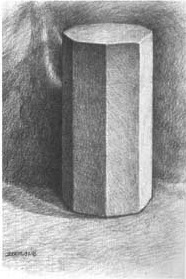
\includegraphics{images/appendix.2.1.jpg}
	\caption*{八棱柱}
\end{figure}

大家是不是对于日记当中那些文字很奇怪呢?那其实是苏格兰古英语来着。。。

ane bouned jew'l of onycs and filigree gold, of finene2s beyond rational ſtatement

a bitter, blaſted place, older than days

a fearſome death god

ſelections of curious providence

可以看到s全部变成了长s:ſ。还有一些几乎无人使用的词语。。。查了好久

古怪的地方:里面说SCP-001不会被任何辐射穿透,但电子显微镜的工作原理就是用辐射穿透物体再观测。。。或许是接受反射回来的辐射的信息吧,毕竟那些黄金是包裹在玛瑙上,突起来的。

现在的宇宙照片大多是个横放的椭球,但这里的南北极点却是相对于一个鸡蛋样子的宇宙来说的:

\begin{figure}[H]
	\centering
	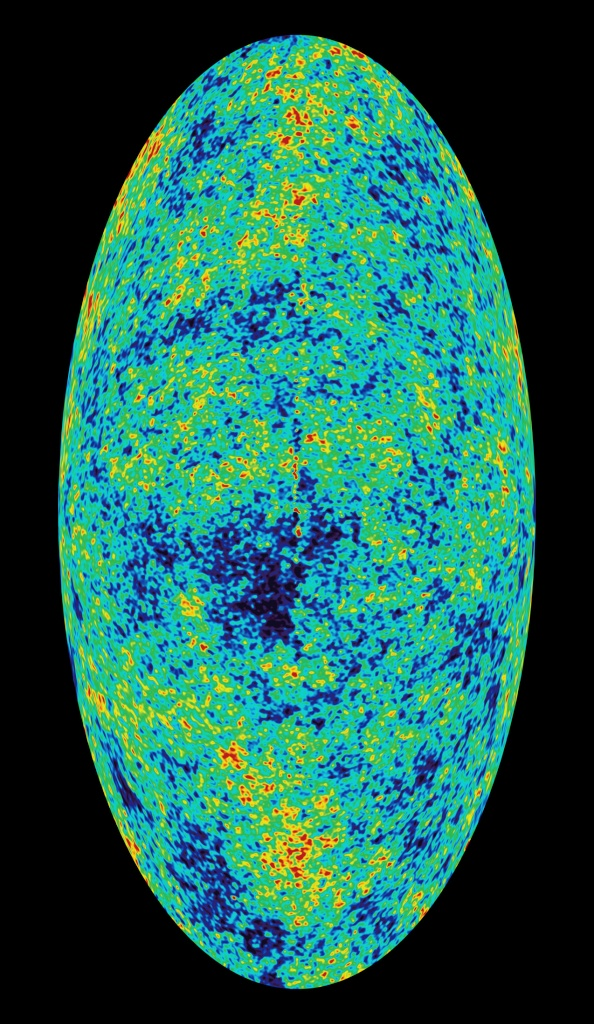
\includegraphics[width=0.5\linewidth]{images/appendix.2.2.jpg}
	\caption*{宇宙微波背景辐射}
\end{figure}

关于宇宙微波背景辐射和温暖:宇宙微波背景辐射(又称3K背景辐射)是一种充满整个宇宙的电磁辐射。频率属于微波范围。是大爆炸后残留下来的余温。在宇宙各处都可以观察到相同的辐射。也就是说,真空是有温度的,大约为-270.15摄氏度。每件物体只要有温度都会放出辐射,只不过冷的物体放出的辐射比其他物体给与它的辐射少,热的东西则相反,所以热量从热到冷流动。而SCP-001完全惰性(这在物理学上是不可能的)又会放出3K辐射,也就是说它不完全接受热量而放出热量,会比所有碰到的物体高3度。人36.5度摸上去就是39.5度,工业炉5000度它对于工业炉就有5003度。所谓温暖实际上是这样引起的。

然后是一个历史知识:苏美尔楔形文字在1400s就已发现,但当时未能破译。直到1802年才由德国教师格罗特芬德破译。再看看馆长翻译的时间:1805……
